% Sección de machine learning de la memoria conjunta del TFM (versión
% divulgativa, 4-5 caras). Autocontenida: pdflatex seccion_ML_divulgativa.tex
% (dos pasadas). Para pegarla en la memoria conjunta basta con copiar desde
% \section hasta el final del documento; el preámbulo solo aporta paquetes
% habituales. Figuras en figs/ (generadas por figs/scripts/).
% El texto es el mismo que seccion_ML_divulgativa.md (09/09/2026).
\documentclass[11pt,a4paper]{article}

\usepackage[T1]{fontenc}
\usepackage[utf8]{inputenc}
% babel-spanish no está instalado en esta máquina; si lo está, añadir
% \usepackage[spanish,es-tabla]{babel} y quitar las dos \renewcommand.
\usepackage{lmodern}
\usepackage[margin=2.2cm]{geometry}
\usepackage{graphicx}
\usepackage{booktabs}
\usepackage{array}
\usepackage{caption}
\usepackage{microtype}
\usepackage{enumitem}
\usepackage[hidelinks]{hyperref}

\graphicspath{{figs/}}
\captionsetup{font=small,labelfont=bf,skip=4pt,width=.92\textwidth}
\setlist{nosep,leftmargin=*}
\setlength{\parskip}{0.2em}
\linespread{0.97}
\setlength{\emergencystretch}{2em}
\renewcommand{\figurename}{Figura}
\renewcommand{\tablename}{Tabla}

\begin{document}

\section{Predicción diaria del riesgo de incendio: dónde y cuándo}
\label{sec:ml}

\subsection{Qué hace este módulo}

La España peninsular cabe en 498.530 celdas de un kilómetro de lado. Este
módulo responde, cada mañana, a una sola pregunta: \textbf{cuáles de esas
celdas van a arder hoy}. No es un mapa de «zonas propensas», que sería el mismo
todos los días, sino una ordenación diaria de las celdas de más a menos
peligro; lo único que importa de ella es si las que efectivamente ardieron
estaban arriba. Es el «antes» del sistema conjunto: anticipa el riesgo que la
visión por computador confirma y que el asistente sobre los partes del MITECO
permite consultar.

El trabajo se hizo dos veces, y esa es su parte más valiosa. Un primer modelo
dio 0,89 de acierto en el laboratorio y, puesto a funcionar cada día,
0,57--0,64. La causa no era el algoritmo ni la meteorología: era que el
conjunto de datos con el que se entrenó hacía otra pregunta. Corregido eso, el
segundo modelo pasa de 0,74 a 0,81 en 2025 y de 0,66 a 0,76 en 2026 sobre las
temporadas completas.

\subsection{Los datos}

Cuatro fuentes, descritas con detalle en el anexo~A:

\begin{itemize}
  \item \textbf{IberFire}, un «cubo» de datos abierto (Tekniker / UPV-EHU) con
  261 variables diarias por celda de 1~km entre 2008 y 2024: tiempo,
  vegetación, terreno, usos del suelo, población, carreteras. De aquí salen
  casi todas las variables.
  \item \textbf{EGIF}, el registro oficial de incendios del Ministerio: una
  fila por incendio con su fecha y el \textbf{punto} de inicio. Etiqueta del
  primer modelo.
  \item \textbf{EFFIS}, los \textbf{perímetros} de superficie quemada que
  Copernicus cartografía por satélite. Etiqueta del segundo modelo y verdad
  contra la que se juzgan los dos.
  \item \textbf{ERA5-Land e IFS} (ECMWF), el reanálisis meteorológico ---lo
  que pasó--- y la previsión ---lo que va a pasar---. Se entrena con lo que
  pasó y se sirve cada día con lo que va a pasar; en el primer modelo, con la
  observación de 687 estaciones de AEMET.
\end{itemize}

De ahí se construyen \textbf{46 variables} por celda y día, en cuatro
familias: \emph{qué tiempo hace} (temperatura, humedad, viento, lluvia de hoy
y de los últimos 7, 15 y 30 días, índice de peligro FWI), \emph{qué hay en la
celda} (bosque, matorral, pendiente, altitud, carreteras, población),
\emph{qué ha ardido cerca antes} (incendios a 1 y 10~km en meses y años
anteriores, focos térmicos de satélite en la última semana) y \emph{qué día
es}.

\paragraph{Lo que enseñó el análisis exploratorio.} Tres cosas que
condicionan todo lo demás. El fuego es rarísimo: en un verano normal arden
entre 2 y 6 celdas de cada 100.000 cada día, y solo el 3~\% de las celdas ha
tenido alguna ignición en seis años. El fuego se agrupa: las celdas quemadas
son contiguas ---perímetros, no puntos---, así que partir los datos al azar
entre entrenamiento y prueba infla el acierto ($+0,036$ medido); todas las
particiones del trabajo son por bloques de 100~km o por años. Y \textbf{el FWI
hay que leerlo en local}: un FWI de 40 es rutina en Almería y excepcional en
Asturias, y lo que separa los días con fuego no es el número sino lo raro que
es \emph{ahí}. El percentil del FWI respecto a la historia de la propia celda
separa mejor que el valor absoluto (mediana 84 en positivos frente a 47 en
negativos) y añadirlo al FWI absoluto aporta $+0,042$ de acierto. Es una aportación propia del trabajo
y la conservan los dos modelos.

\subsection{Primer modelo: entrenamiento y evaluación}

El primer modelo se construyó como se construyen casi todos los de la
literatura. Los positivos son los 19.561 incendios del registro EGIF de 2015 a
2020, cada uno en su celda y su fecha. Los negativos se sortean tomando
\textbf{la misma celda en otros días} en que no ardió, tres por cada positivo.
Se entrena un XGBoost, se afina con 2021 y se prueba con 2022, el peor año de
la década, con Losacio y Sierra de la Culebra dentro. Resultado: \textbf{AUC
0,89}, sin fugas (con las etiquetas barajadas cae al azar) y sin colapso al
validarlo por bloques espaciales de 100~km. Afinar los parámetros añadía $+0,007$: el
rendimiento estaba en las variables, no en el ajuste.

Con ese resultado se puso en producción en julio de 2026: cada mañana descarga
la observación de las 687 estaciones, calcula las 46 variables y publica un
ranking nacional y un mapa de riesgo para hoy y mañana. Desde entonces corre a
diario, y esa serie sellada es lo que permite lo que sigue.

Y entonces se midió contra la realidad: contra los perímetros de EFFIS, contra
los partes diarios del MITECO y contra los focos térmicos de satélite. El
acierto diario del modelo en producción estuvo entre \textbf{0,57 y 0,64}. Un
índice sin modelo, el percentil local del FWI a secas, sacaba 0,70.

Había tres sospechosos, y los dos primeros se descartaron con números:

\begin{enumerate}
  \item \textbf{¿Está mal medido?} No: tres verdades independientes
  ---satélite, cartografía y partes oficiales--- cuentan lo mismo.
  \item \textbf{¿Es la meteorología?} El modelo se entrenó con el reanálisis
  del cubo y se sirve con estaciones. Hay diferencias reales ---el reanálisis
  «llueve» 8~mm más al mes y eso baja el FWI 10 puntos---, pero cuantificadas
  no explican la caída. Tampoco lo que cambia entre entrenar y servir:
  sustituir las variables de satélite por su climatología cuesta 0,0045.
  \item \textbf{Es la pregunta.} Al sortear los negativos en \emph{la misma
  celda otros días}, el 98,8~\% de las celdas de la muestra tenían
  exactamente un 25~\% de días con fuego. El modelo no podía aprender
  qué celda es más peligrosa que otra, porque todas tenían la misma
  proporción; solo podía aprender \textbf{qué día} es peligroso. Respondía a
  «¿es hoy un día malo en esta celda?» y en operación se le preguntaba «¿cuál
  de las 498.530 celdas arde hoy?».
\end{enumerate}

\subsection{Segundo modelo: cambiar la pregunta, no el algoritmo}

La figura~\ref{fig:disenios} resume el problema y la solución. En el primer
diseño (a) cada celda quemada se compara consigo misma en otros días; en el
segundo (b) se compara con otras celdas del mismo día, que es exactamente lo
que se pide en operación (c). La prueba de que esto es lo que fallaba es que
la métrica de laboratorio era ciega a la diferencia: dos conjuntos de
entrenamiento, uno con cada diseño, dan \textbf{0,92 los dos} medidos cada uno
con su propio banco de pruebas; medidos \textbf{dentro de cada día}, como se
usan, dan 0,744 y 0,828.

\begin{figure}[htbp]
  \centering
  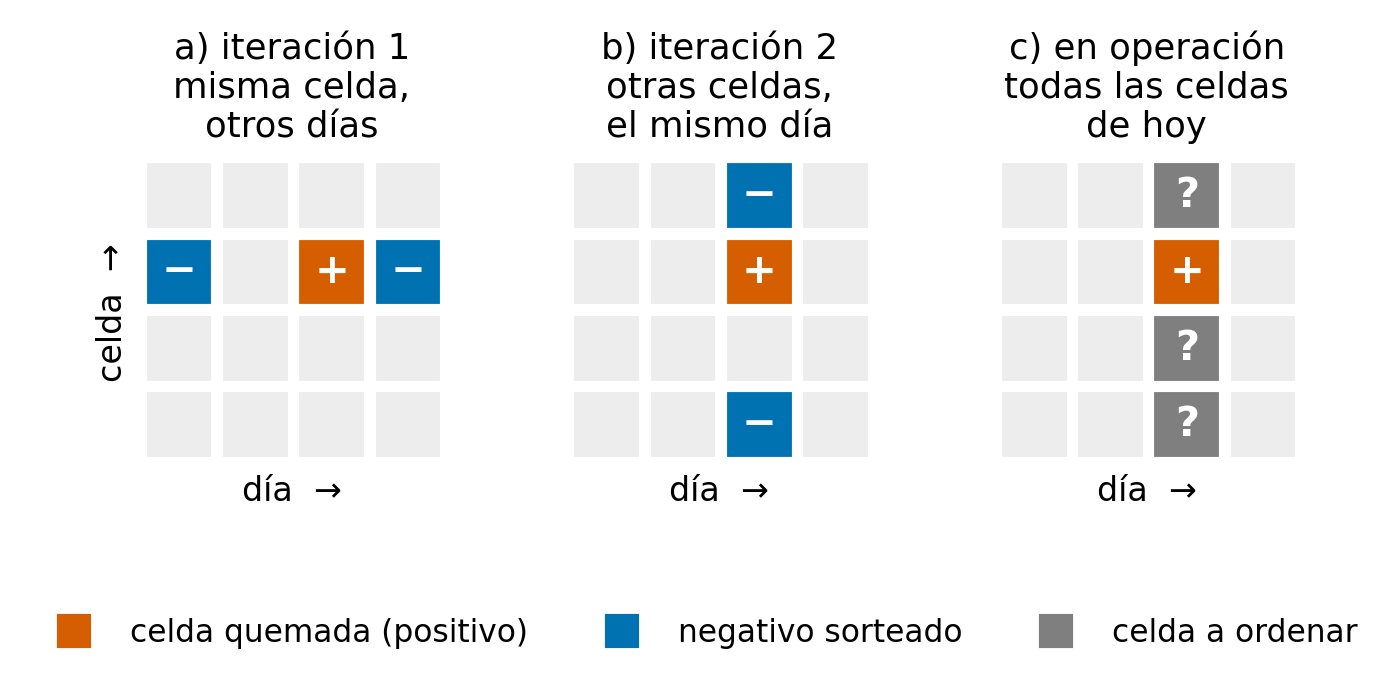
\includegraphics[width=.62\textwidth]{f2_disenios.png}
  \caption{La misma rejilla celda~$\times$~día con los dos diseños de muestreo
  y la pregunta operativa. (a)~Iteración~1: para cada celda quemada, los
  negativos son \emph{la misma celda en otros días}; el modelo solo puede
  aprender qué día es peligroso. (b)~Iteración~2: los negativos son
  \emph{otras celdas del mismo día}; el modelo aprende a comparar celdas.
  (c)~Lo que se pide cada mañana: ordenar todas las celdas de hoy. Solo (b)
  hace la misma pregunta que (c).}
  \label{fig:disenios}
\end{figure}

La segunda versión cambia exactamente dos cosas y deja lo demás igual: las
mismas 46 variables, el mismo algoritmo con los mismos parámetros, la misma
malla. \textbf{Los negativos son otras celdas del mismo día}, y \textbf{la
etiqueta es la superficie quemada de EFFIS}, la misma con la que se juzga
---entrenar con puntos de ignición y evaluar con perímetros era comparar dos
cosas distintas: solo el 15~\% de las igniciones de 25--100~ha coincide celda
a celda con un perímetro del mismo día---. Se entrena con 2015--2022, se afina
con 2023 y se prueba con 2024, siempre dentro de cada día. Se compararon un
modelo único frente a la pareja de un \emph{dónde} (fijo) por un
\emph{cuándo} (diario), y distintas cantidades de negativos por positivo. Se
eligió el \textbf{modelo único con diez negativos por positivo}, «r10» en
adelante: la cantidad de negativos mueve el acierto medio apenas $+0,01$, del
orden del azar del sorteo, y en la temporada de 2026 el 1:10 fue el que mejor
situó los incendios grandes, que es donde importa. Las pruebas que salieron mal ---entrenar solo
con verano empeora, añadir una capa de «ya quemado» empeora--- están en el
anexo~B.

Antes de dar por bueno un modelo conviene mirar en qué se fija, y que cuadre
con lo que se sabe del fuego (figura~\ref{fig:shap}). Lo que más pesa es el
\textbf{historial}: cuántos incendios ha habido a 10~km en ese mismo mes en
años anteriores. Después el \textbf{combustible} ---verdor acumulado en el
último mes, matorral, pendiente--- y el \textbf{tiempo}: humedad mínima baja y
FWI anómalo para la celda empujan hacia arriba; suelo agrícola y lluvia
reciente, hacia abajo. Es el retrato que daría un técnico de extinción, con un
matiz: el verdor y la temperatura de superficie \emph{del propio día} llevan
ya parte de la firma del incendio en el cubo (pesan un 4~\% del modelo) y en
servicio se sustituyen por su climatología mensual.

\begin{figure}[htbp]
  \centering
  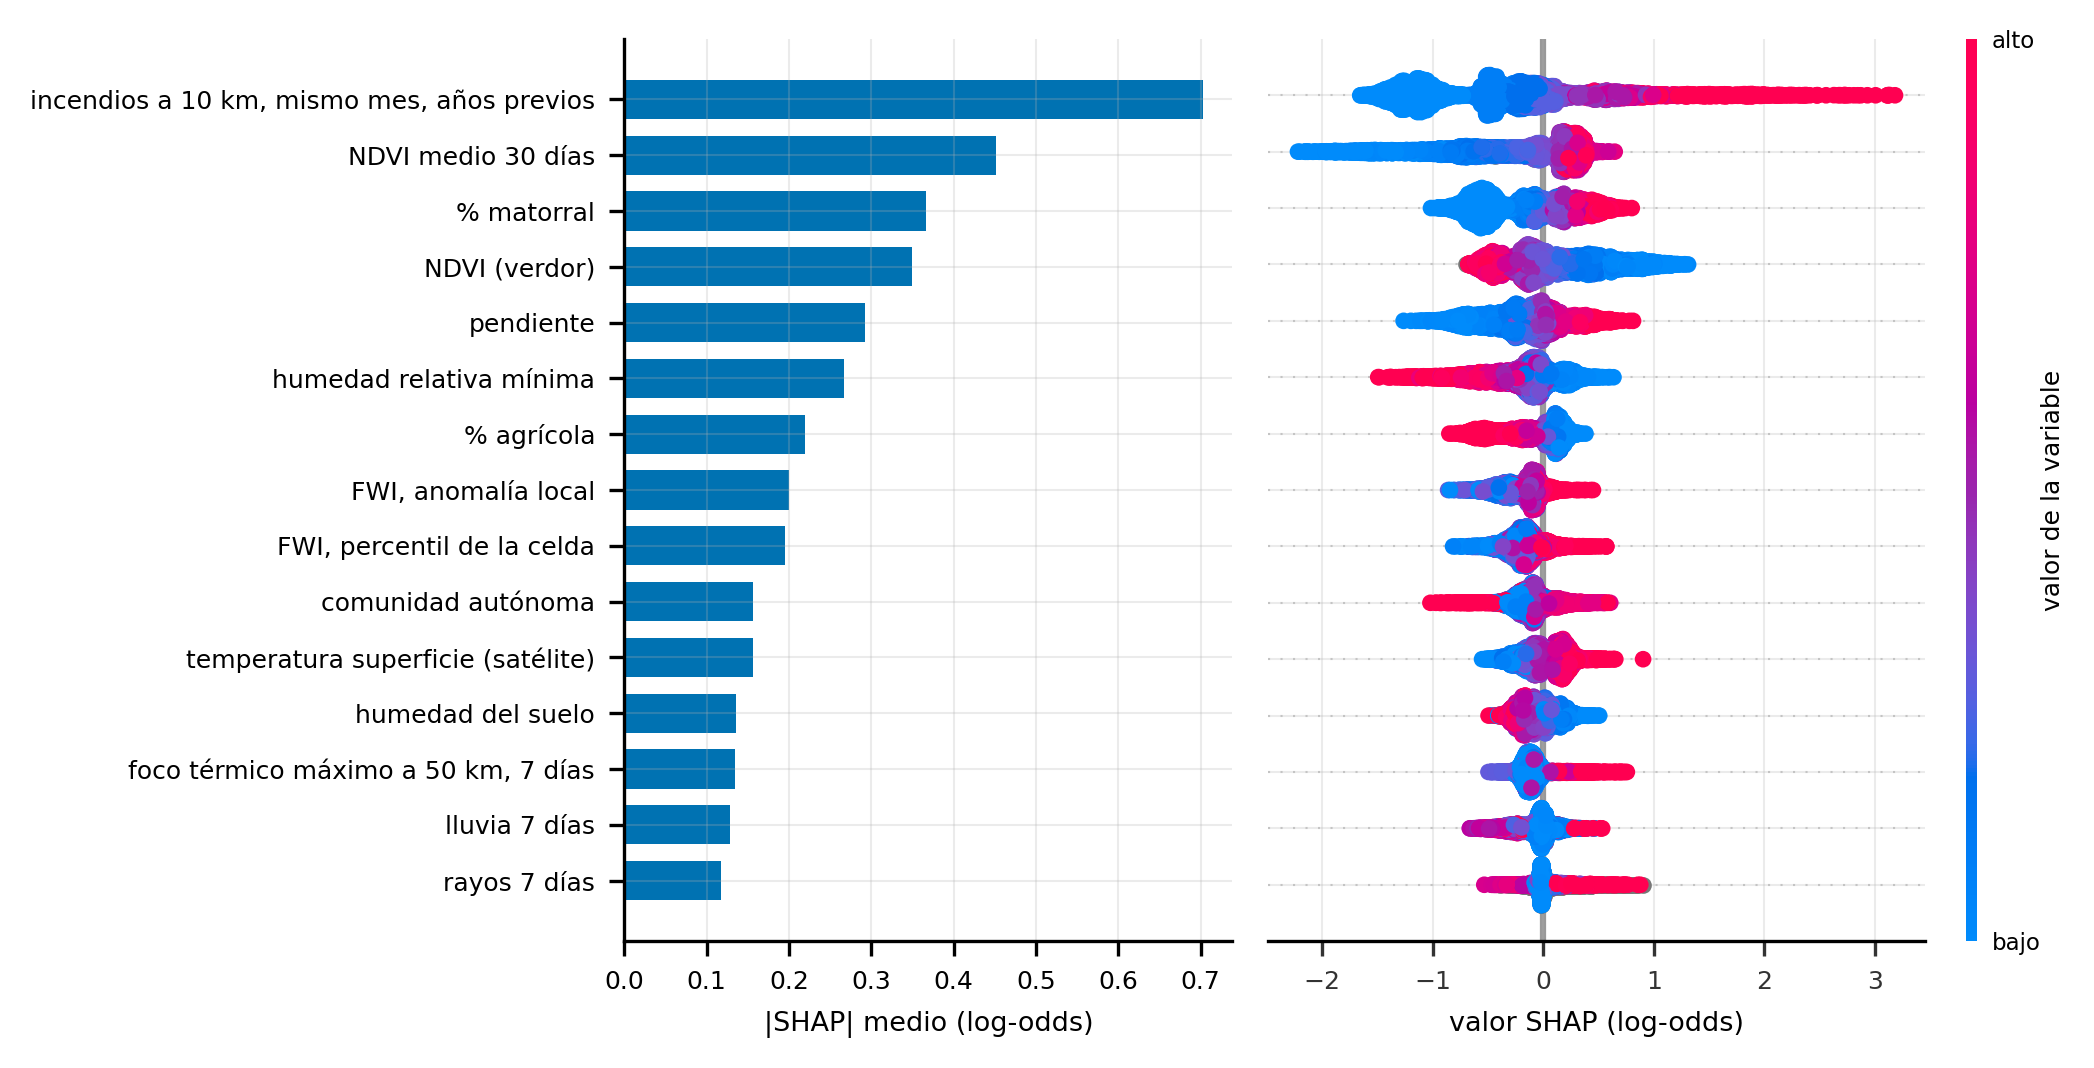
\includegraphics[width=.68\textwidth]{f11_shap_r10.png}
  \caption{Qué mira el r10: las 15 variables de mayor peso por valores SHAP
  sobre 6.000 celdas-día de los veranos de 2023 y 2024, que el modelo no vio
  al entrenar. Izquierda, importancia media; derecha, el efecto de cada fila
  (a la derecha del cero, empuja el riesgo hacia arriba) con el valor de la
  variable en color (rojo, alto). Historial de fuego, combustible y sequedad,
  por ese orden.}
  \label{fig:shap}
\end{figure}

\subsection{Resultados, límites y conclusiones}

Para comparar con justicia hay que poner a los dos modelos ante los mismos
días, la misma meteorología y la misma verdad. Se reprodujeron día a día las
temporadas de 2025 (1 de junio a 1 de noviembre) y 2026 (hasta el 2 de
septiembre), alimentando a ambos con \textbf{la previsión disponible la
víspera} y juzgándolos con los perímetros de EFFIS
(tabla~\ref{tab:replay}). El protocolo se escribió antes de ejecutar nada.

\begin{table}[htbp]
  \centering
  \caption{Acierto medio por día (AUC dentro del día) de producción y del r10
  con la previsión de la víspera, juzgados con EFFIS. La diferencia es la
  media pareada día a día, con intervalo bootstrap al 95~\%.}
  \label{tab:replay}
  \footnotesize
  \begin{tabular}{lrrrrcr}
    \toprule
    Temporada & Días con fuego & Hectáreas & Producción & r10 & Diferencia (IC~95~\%) & Gana el r10 \\
    \midrule
    2025 & 138 & 387.000 & 0,743 & \textbf{0,807} & $+0,064$ [$+0,027$, $+0,101$] & 60~\% \\
    2026 &  86 & 268.000 & 0,658 & \textbf{0,762} & $+0,104$ [$+0,065$, $+0,144$] & 67~\% \\
    \bottomrule
  \end{tabular}
\end{table}

Tres lecturas. \textbf{La mejora no es ruido}: el intervalo no toca el cero en
ninguna temporada y el r10 gana dos de cada tres días, más en 2026, cuando
producción lo pasó peor. \textbf{Predecir no cuesta nada}: cada día se calculó
con la previsión de la víspera y con el tiempo que realmente hizo, y la
diferencia es $-0,003$; el modelo no depende de acertar el tiempo al detalle
sino de saber dónde está el combustible y cuánto lleva seco. \textbf{Es un
mapa para vigilar, no una alarma por celda}: que arda una celda concreta un
día concreto es una de cada diez mil, y el mapa dice dónde mirar, no dónde va
a arder. El sistema corre además en vivo desde el 21 de agosto contra tres
jueces diarios; el r10 va por delante, pero con pocos días los intervalos aún
cruzan el cero (anexo~C).

\paragraph{Del ranking al producto.} El mapa se pintaba por posición en el
ranking del día ---el 2~\% más alto en rojo---, y el ranking siempre tiene un
primero: un martes de febrero sale con tanto rojo como el 15 de agosto. La
solución tiene dos piezas (figura~\ref{fig:escala}). La primera es fijar los
colores \textbf{en la escala de la nota}: se pasaron los modelos por los diez
años del cubo y se anotó a partir de qué nota se entra en el 2~\% más alto
\emph{de toda la historia}; con esa regla, de cada 800 celdas pintadas de
EXTREMO en diez años ardió una, 36 veces el promedio. La segunda es un
\textbf{semáforo nacional}: si la nota del 2~\% más alto de España ese día no supera el
umbral que en la historia separa los días con incendio grande, hoy no es día
de fuego y el mapa no se pinta. Con esa puerta, en invierno el 44~\% de los
días quedan sin rojo perdiendo el 6~\% de los días grandes. El semáforo tiene
habilidad fuera de temporada y ninguna en verano, cuando casi todos los días
pasan del umbral: en verano manda el mapa, en invierno el semáforo evita el
rojo falso. La nota \textbf{no es una probabilidad}: es una puntuación para
ordenar y comparar con umbrales, y así se presenta.

\begin{figure}[htbp]
  \centering
  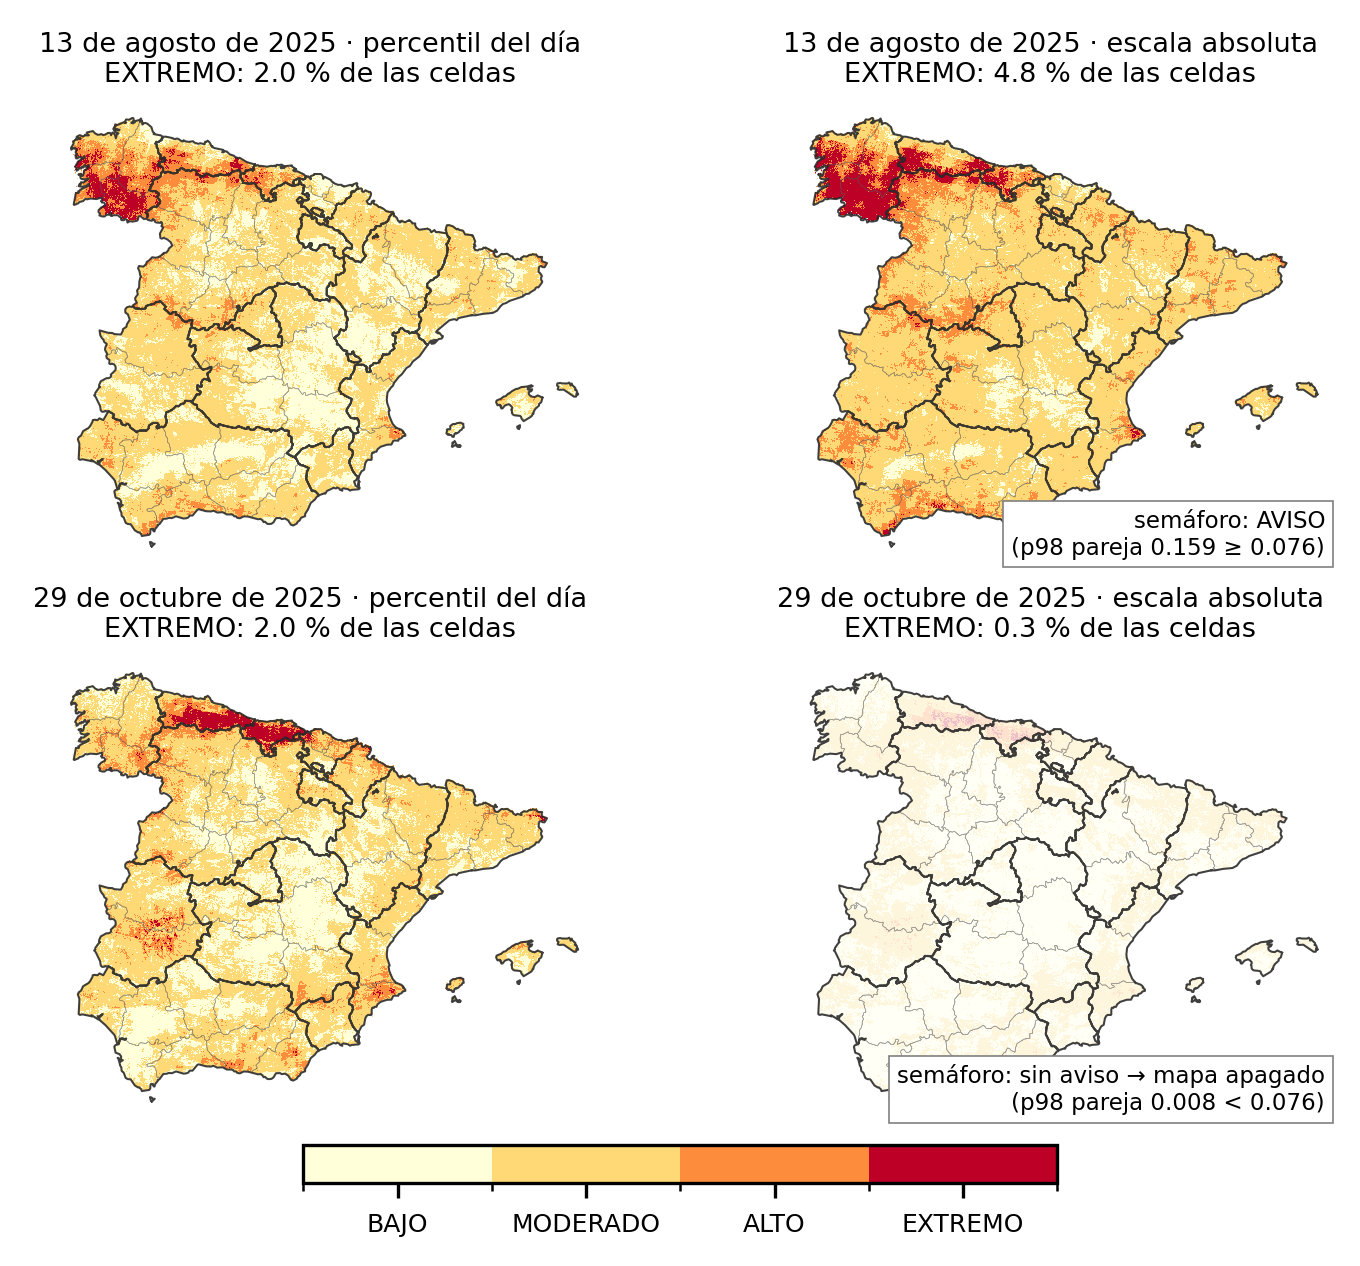
\includegraphics[width=.5\textwidth]{f10_percentil_vs_absoluto.png}
  \caption{El mismo modelo (r10) pintado de dos maneras en un día de pleno
  verano (13 de agosto de 2025, arriba) y en uno fuera de temporada (29 de
  octubre de 2025, abajo). Izquierda: niveles por percentil del día, que
  reparten el 2~\% de EXTREMO cada día sin excepción. Derecha: cortes fijos en
  la escala de la nota, aprendidos de diez años de historia, y el semáforo
  nacional: el 29 de octubre no supera el umbral y el mapa se apaga.}
  \label{fig:escala}
\end{figure}

\paragraph{Límites.} La evaluación de dos temporadas es a posteriori: los
mapas usan la previsión de cada víspera, pero se generaron después, no
sellados día a día; lo sellado es la cadena en vivo, que aún tiene pocos días.
La producción sirve una versión con un defecto conocido en el cálculo del
viento, no corregido a propósito para no romper la comparación (anexo~E).
Cobertura: Península y Baleares, sin Canarias; datos de 2026 hasta el 2 de
septiembre.

\paragraph{Conclusión.} Un modelo se optimiza para la pregunta que define su
conjunto de entrenamiento, y esa pregunta la fija la elección de positivos y
negativos, no la intención de quien lo entrena. Un acierto alto sobre un banco
construido con el mismo diseño que el entrenamiento no demuestra nada sobre el
uso previsto. La comprobación que lo detecta ---evaluar dentro de cada día,
con la misma verdad con la que se va a juzgar el sistema--- es barata y
debería hacerse antes de entrenar, no después de dos meses en producción. El
código, con cada cifra enlazada a su script, está en el repositorio
(anexo~F).

\end{document}
